% Für Arbeiten auf Deutsch
\documentclass[deutsch,oribibl,a4paper]{llncs}
\usepackage{ngerman}
\usepackage[utf8]{inputenc}

% Bitte bindet keine .eps-Dateinen als Bilder ein (do not use \usepackage{epsfig}!)
\usepackage{graphicx}

%Wer lieber mit Postscript-Ausgaben arbeitet, muss dieses Packet auskommentieren
\usepackage[pdftex,
						colorlinks=true, linkcolor=blue, urlcolor=cyan, citecolor=red,%
						raiselinks=true,%
            bookmarks=true,%
            bookmarksopenlevel=1,%
            bookmarksopen=true,%
            bookmarksnumbered=true,%
            hyperindex=true,% 
            plainpages=false,% correct hyperlinks
            pdfpagelabels=true%,% view TeX pagenumber in PDF reader
            colorlinks=false,
            citecolor=black,
            %pdfborder={0 0 0.5}
            ]{hyperref} % erzeuge Hyperlinks z.B. für pdflatex

% Wer mit eigenen Farben arbeiten möchte
\usepackage{color}
\definecolor{darkgreen}{rgb}{0.23,0.46,0.23}

% Mit diesem Package kann man sich elegant eigene Codeumgebungen definieren
\usepackage{textcomp}
\usepackage{listings} 
\lstdefinelanguage{QVTrelation}{
		%alsoletter={-,=},
		morekeywords={transformation,key,top,relation,checkonly,enforce,domain,when,where,or,and},
		tabsize=2,
		frame=single,
		upquote=true, % how the upper quotes are displayed '
		%showspaces=true,
		basicstyle=\ttfamily \scriptsize,
		morecomment=[s][\color{darkgreen}]{/*}{*/},
		%commentstyle=\color{green},
    keywordstyle=\color{blue} \bfseries,
    %language=XML,
    escapeinside={\%}{\%},
    numbers=left,  
    numberfirstline=true,
    firstnumber=1,
    numberstyle=\scriptsize, 
    numbersep=5pt
    } 
\lstnewenvironment{QVTrelation}[2]
		{\lstset{language=QVTrelation, numbers=left, stepnumber=2, caption={#1}, label={#2}}}
		{}   

\pagestyle{plain}
\begin{document}

%Anpassen!
\title{Bio-inspired \& Grid Computing I}
\subtitle{Seminar Software Engineering verteilter Systeme\\ Sommersemester 2015}

\author{Holger Kasinger\\ Matrikelnummer: XXXXXXXX \\ \email{kasinger@informatik.uni-augsburg.de}}

\institute{Betreuer: Chuck Norris\\ Professur Softwaremethodik für verteilte Systeme (Prof. Bauer)\\ Universität Augsburg}


\maketitle

%Ab hier beginnt die Schreibarbeit ...
\begin{abstract}
	Lorem ipsum dolor sit amet, consectetuer adipiscing elit, sed diam nonummy nibh euismod tincidunt ut laoreet dolore magna aliquam erat volutpat. Ut wisi enim ad minim veniam, quis nostrud exerci tation ullamcorper suscipit lobortis nisl ut aliquip ex ea commodo consequat.
\end{abstract}

%Inhaltsverzeichnis ist nur für die Besprechungen. Für die endgültige Version auskommentieren.
%\tableofcontents

\newpage

\section{Einleitung}
\label{sec:Einleitung}
\cite{Konak2006,Sailer2013} and \cite{01_MW-Paper}


\section{Hauptteil}
\label{sec:Hauptteil}

TEXT

\begin{figure}[htb]
	\centering
		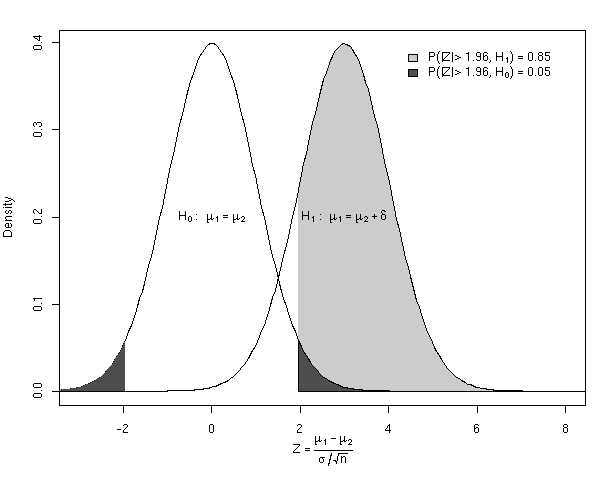
\includegraphics[width=0.75\textwidth]{power.png}
	\caption{Beispielabbildung}
	\label{fig:power}{}		
\end{figure}

TEXT

\subsection{Erste Zwischenüberschrift}
\label{sec:ErsteZwischenueberschrift}

TEXT

\begin{QVTrelation}{Ein Codebeispiel}{QVTlist1} 
transformation MMa2MMb(ma:MMa; mb:MMb) {

/* Dies ist ein Kommentar */

	key MMb::Library{name}; 

%$\Rightarrow$ mit \% kann man wieder in die normal Latex-Umgebung wechseln%
	
	top relation LibraryToLibrary {
		n: String;
		checkonly domain ma c:Library {name=n};
		enforce domain mb c_:Library {name=n};
	}
	
	top relation NovelToNovel {
		i, n: String;
		checkonly domain ma c:Novel {ns=l:Library{},name=n,index=i} ;
		enforce domain mb c_:Novel {ns=l_:Library{},name=n,index=i} ;
		when {
			LibraryToLibrary(l,l_);
		}		
		where {
			AuthorsToAuthors(c,c_);
		}
	}
}
\end{QVTrelation}

TEXT

\subsubsection{Erste Unterüberschrift}
\label{sec:ErsteUnterueberschrift}

TEXT

\subsection{Zweite Zwischenüberschrift}
\label{sec:ZweiteZwischenueberschrift}

TEXT

\section{Schluss}
\label{sec:Schluss}

TEXT

%Bibliography
\bibliographystyle{alpha}
\bibliography{literature}


% Alles was nicht direkt in die Arbeit soll (optional) und die Eidesstattliche Erklärung (anpassen!)
\begin{appendix}
% Platz für den Anhang (optional)
\end{appendix}
%%% Local Variables:
%%% mode: latex
%%% TeX-master: "Seminararbeit"
%%% End:


\end{document}
